\documentclass[10pt, a4paper]{article} % 设置字体大小和纸张类型
\usepackage{fontspec}
\setmainfont{Times New Roman}

\usepackage{booktabs} % 支持更专业的表格线条
\usepackage{ctex}
\usepackage{caption} % 插图和表格的标题格式
\usepackage{amsmath, amsfonts, amssymb} % 数学公式支持
\usepackage{graphicx} % 插入图片
\usepackage{hyperref} % 超链接支持
\usepackage{hypcap} % 修正超链接指向的图片位置
\usepackage{geometry}
\usepackage{titlesec}
\usepackage{fmtcount} % 用于数字到中文的转换
\usepackage{enumitem} % 加载 enumitem 宏包
\usepackage{multirow} % 支持多行单元格
\usepackage{diagbox}
\usepackage{makecell} % 支持单元格内换行
\usepackage{tikz}
\usepackage{makecell}
\usepackage{unicode-math}
\setmathfont{Latin Modern Math}



\renewcommand{\thesection}{\chinese{section}、}
\renewcommand{\thesubsection}{\arabic{subsection}.}


\begin{document}

\begin{titlepage}
    \newgeometry{left=0cm, right=0cm, top=0cm, bottom=0cm}
    \centering
    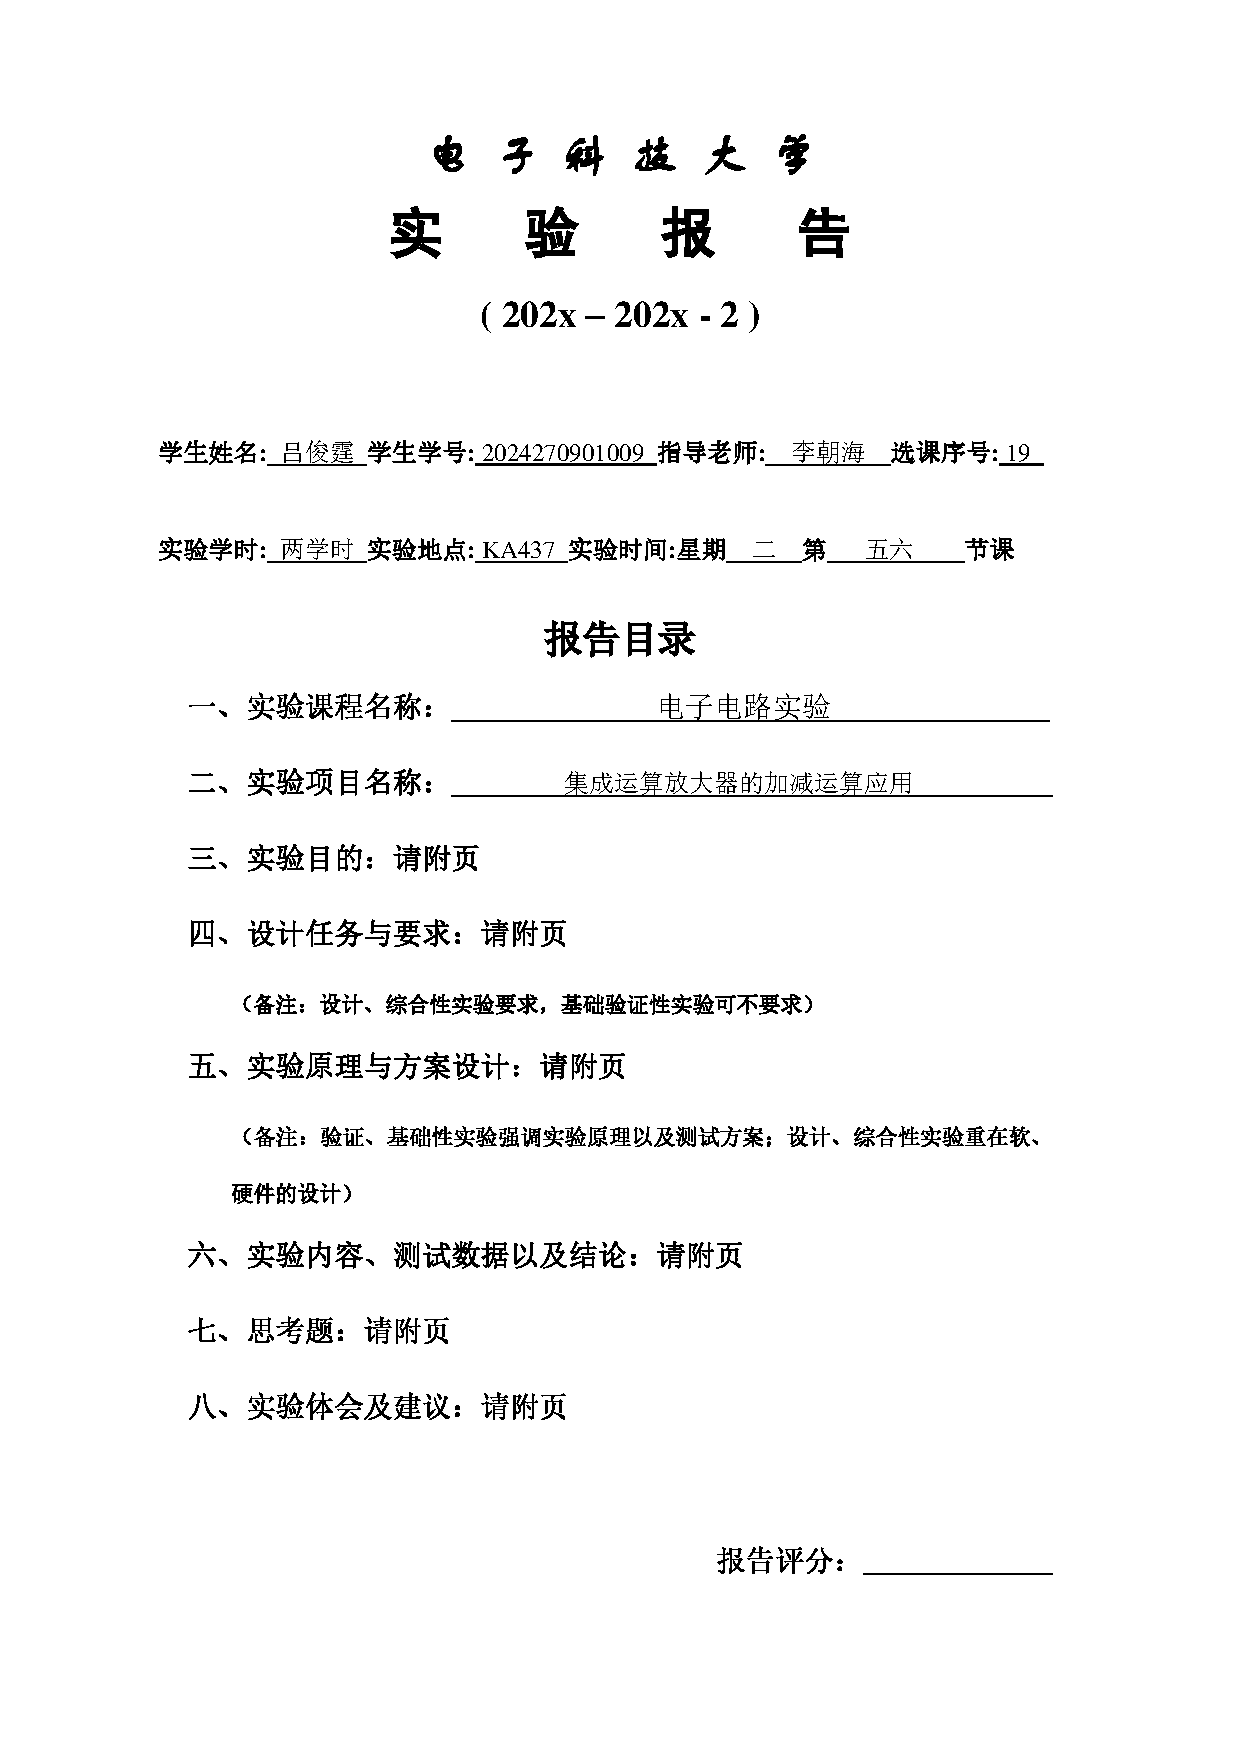
\includegraphics[page=1, width=0.9\textwidth, keepaspectratio]{image/实验报告撰写封面.pdf}
    \restoregeometry
\end{titlepage}

\setcounter{section}{2}

\section{实验目的}

\begin{enumerate}[leftmargin=50pt,label=(\arabic*)] % 设置序号格式为(1)
    \item 进一步理解集成运放的基本特性
    \item 熟练掌握集成运放的正确使用方法
    \item 理解加法器、减法器原理及其实际应用
    \item 应用示波器测量技术对运放的运算关系进行研究
\end{enumerate}

\section{设计任务与要求}

暂不需要。

\section{实验原理与方案设计}
\subsection{实验原理}
\textbf{(1)加法运算电路}

实际中经常遇到需对模拟信号进行代数相加的应用,完成这一运算的电路有反相加法器和同相加法器。如图~\hyperref[fig:加法器电路图]{\ref{fig:加法器电路图}}所示,在反相比例放大电路的基础上,增加一个或多个输入支路,就构成了反相加法运算电路,此时多个输入信号电压产生的电流都流向$R_f$,所以输出是多个输入信号的和。根据“虚短”和“虚断”的结论可得
$$
u_- = u_+ = 0 i_1 + i_2 = i_f
$$
因为 
$$
i_1 = \frac{v_{11}}{R_1}, i_2 = \frac{v_{12}}{R_2}, i_f = -\frac{v_o}{R_f}
$$
则
$$
\frac{v_{11}}{R_1} + \frac{v_{12}}{R_2} = -\frac{v_o}{R_f}
$$
$$
v_o = -R_f \left( \frac{v_{11}}{R_1} + \frac{v_{12}}{R_2} \right)
$$
若取
$$
R_1 = R_2 = R
$$
则有
$$
v_o = -\frac{R_f}{R} \left( v_{11} + v_{12} \right)
$$

同相加法器是在同相比例放大电路的基础上,增加一个或多个输入支路来构成同相输入求和电路,因运放具有“虚断”的特性,对运放同相输入端的电位可用叠加原理求得。
\clearpage
\textbf{(2)减法运算电路}

减法器又称为差分放大电路,即集成运放再两个输入端同时输入信号的情况下,在输出端得到两个模拟信号相减的运算结果。减法运算电路如图~\hyperref[fig:减法器电路图]{\ref{fig:减法器电路图}}所示,一路信号送入反相输入端,另一路信号接到同相输入端。根据“虚短”和“虚断”的结论可得
$$
v_{-} = v_{+} = \frac{R_3}{R_2+R_3}v_{12}  
i_1 = i_f
$$
而
$$
i_1 = \frac{v_{11}-\frac{R_3}{R_2+R_3}v_12}{R_1} 
i_f = \frac{\frac{R_3}{R_2+R_3}V_{12} - v_o}{R_f}
$$
所以
$$
v_O = \frac{R_3}{R_1}\cdot\frac{R_1+R_f}{R_2+R_3}v_{12} - \frac{R_f}{R_1}v_{11} 
$$
若取
$$
R_1 = R_2 \& R_3=R_f
$$
则有
$$
v_o = \frac{R_f}{R_1}\left( v_{12} - v_{11} \right)
$$

\begin{figure}[htbp]
    
    \centering
    \begin{minipage}
{0.45\textwidth}
        \centering
        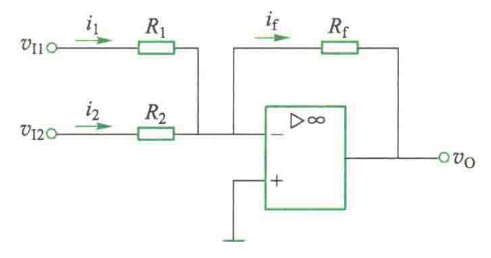
\includegraphics[width=1.0\textwidth]{image/1.png}
        \caption{加法器电路图}
        \label{fig:加法器电路图}
    \end{minipage}
    \hfill
    \begin{minipage}
{0.45\textwidth}
        \centering
        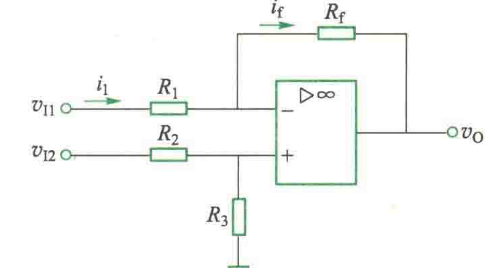
\includegraphics[width=1.0\textwidth]{image/2.png}
        \caption{减法器电路图}
        \label{fig:减法器电路图}
    \end{minipage}
\end{figure}

\section{实验内容、测试数据以及结论}

\subsection{实验内容}
\textbf{(1)反相加法器的设计与测试}

\begin{tabular}{|c|c|c|c|c|}
    \hline
    \multicolumn{2}{|c|}{\textbf{测试条件}} & \multicolumn{2}{c|}{\textbf{所选电阻大小}} & \textbf{输出电压} \\
    \multicolumn{2}{|c|}{} &  \multicolumn{2}{|c|}{}  &(写出表达式并定量绘出波形) \\ \hline
    $v_{11}/V$ & $v_{12}/V$ & $R_1/\Omega$ & $R_f/\Omega$ & $v_o/V$ \\ \hline
    $\cos(1000\pi t)$ & 0.7 &10K&30K& \\ \hline
\end{tabular}
\clearpage

\textbf{(2)同相加法器的设计与测试}

\begin{tabular}{|c|c|c|c|c|}
    \hline
    \multicolumn{2}{|c|}{\textbf{测试条件}} & \multicolumn{2}{c|}{\textbf{所选电阻大小}} & \textbf{输出电压} \\
    
     \multicolumn{2}{|c|}{} &  \multicolumn{2}{|c|}{}  & (写出表达式并定量绘出波形) \\
    \hline
    $v_{11}/V$ & $v_{12}/V$ & $R_1/\Omega$& $R_f/\Omega$& $v_o/V$ \\
    \hline
    $\cos(1000\pi t)$ & 0.7 &10K&30K& \\
    \hline
\end{tabular}

\begin{figure}[ht]
    
        \centering
        \begin{minipage}
    {0.45\textwidth}
            \centering
            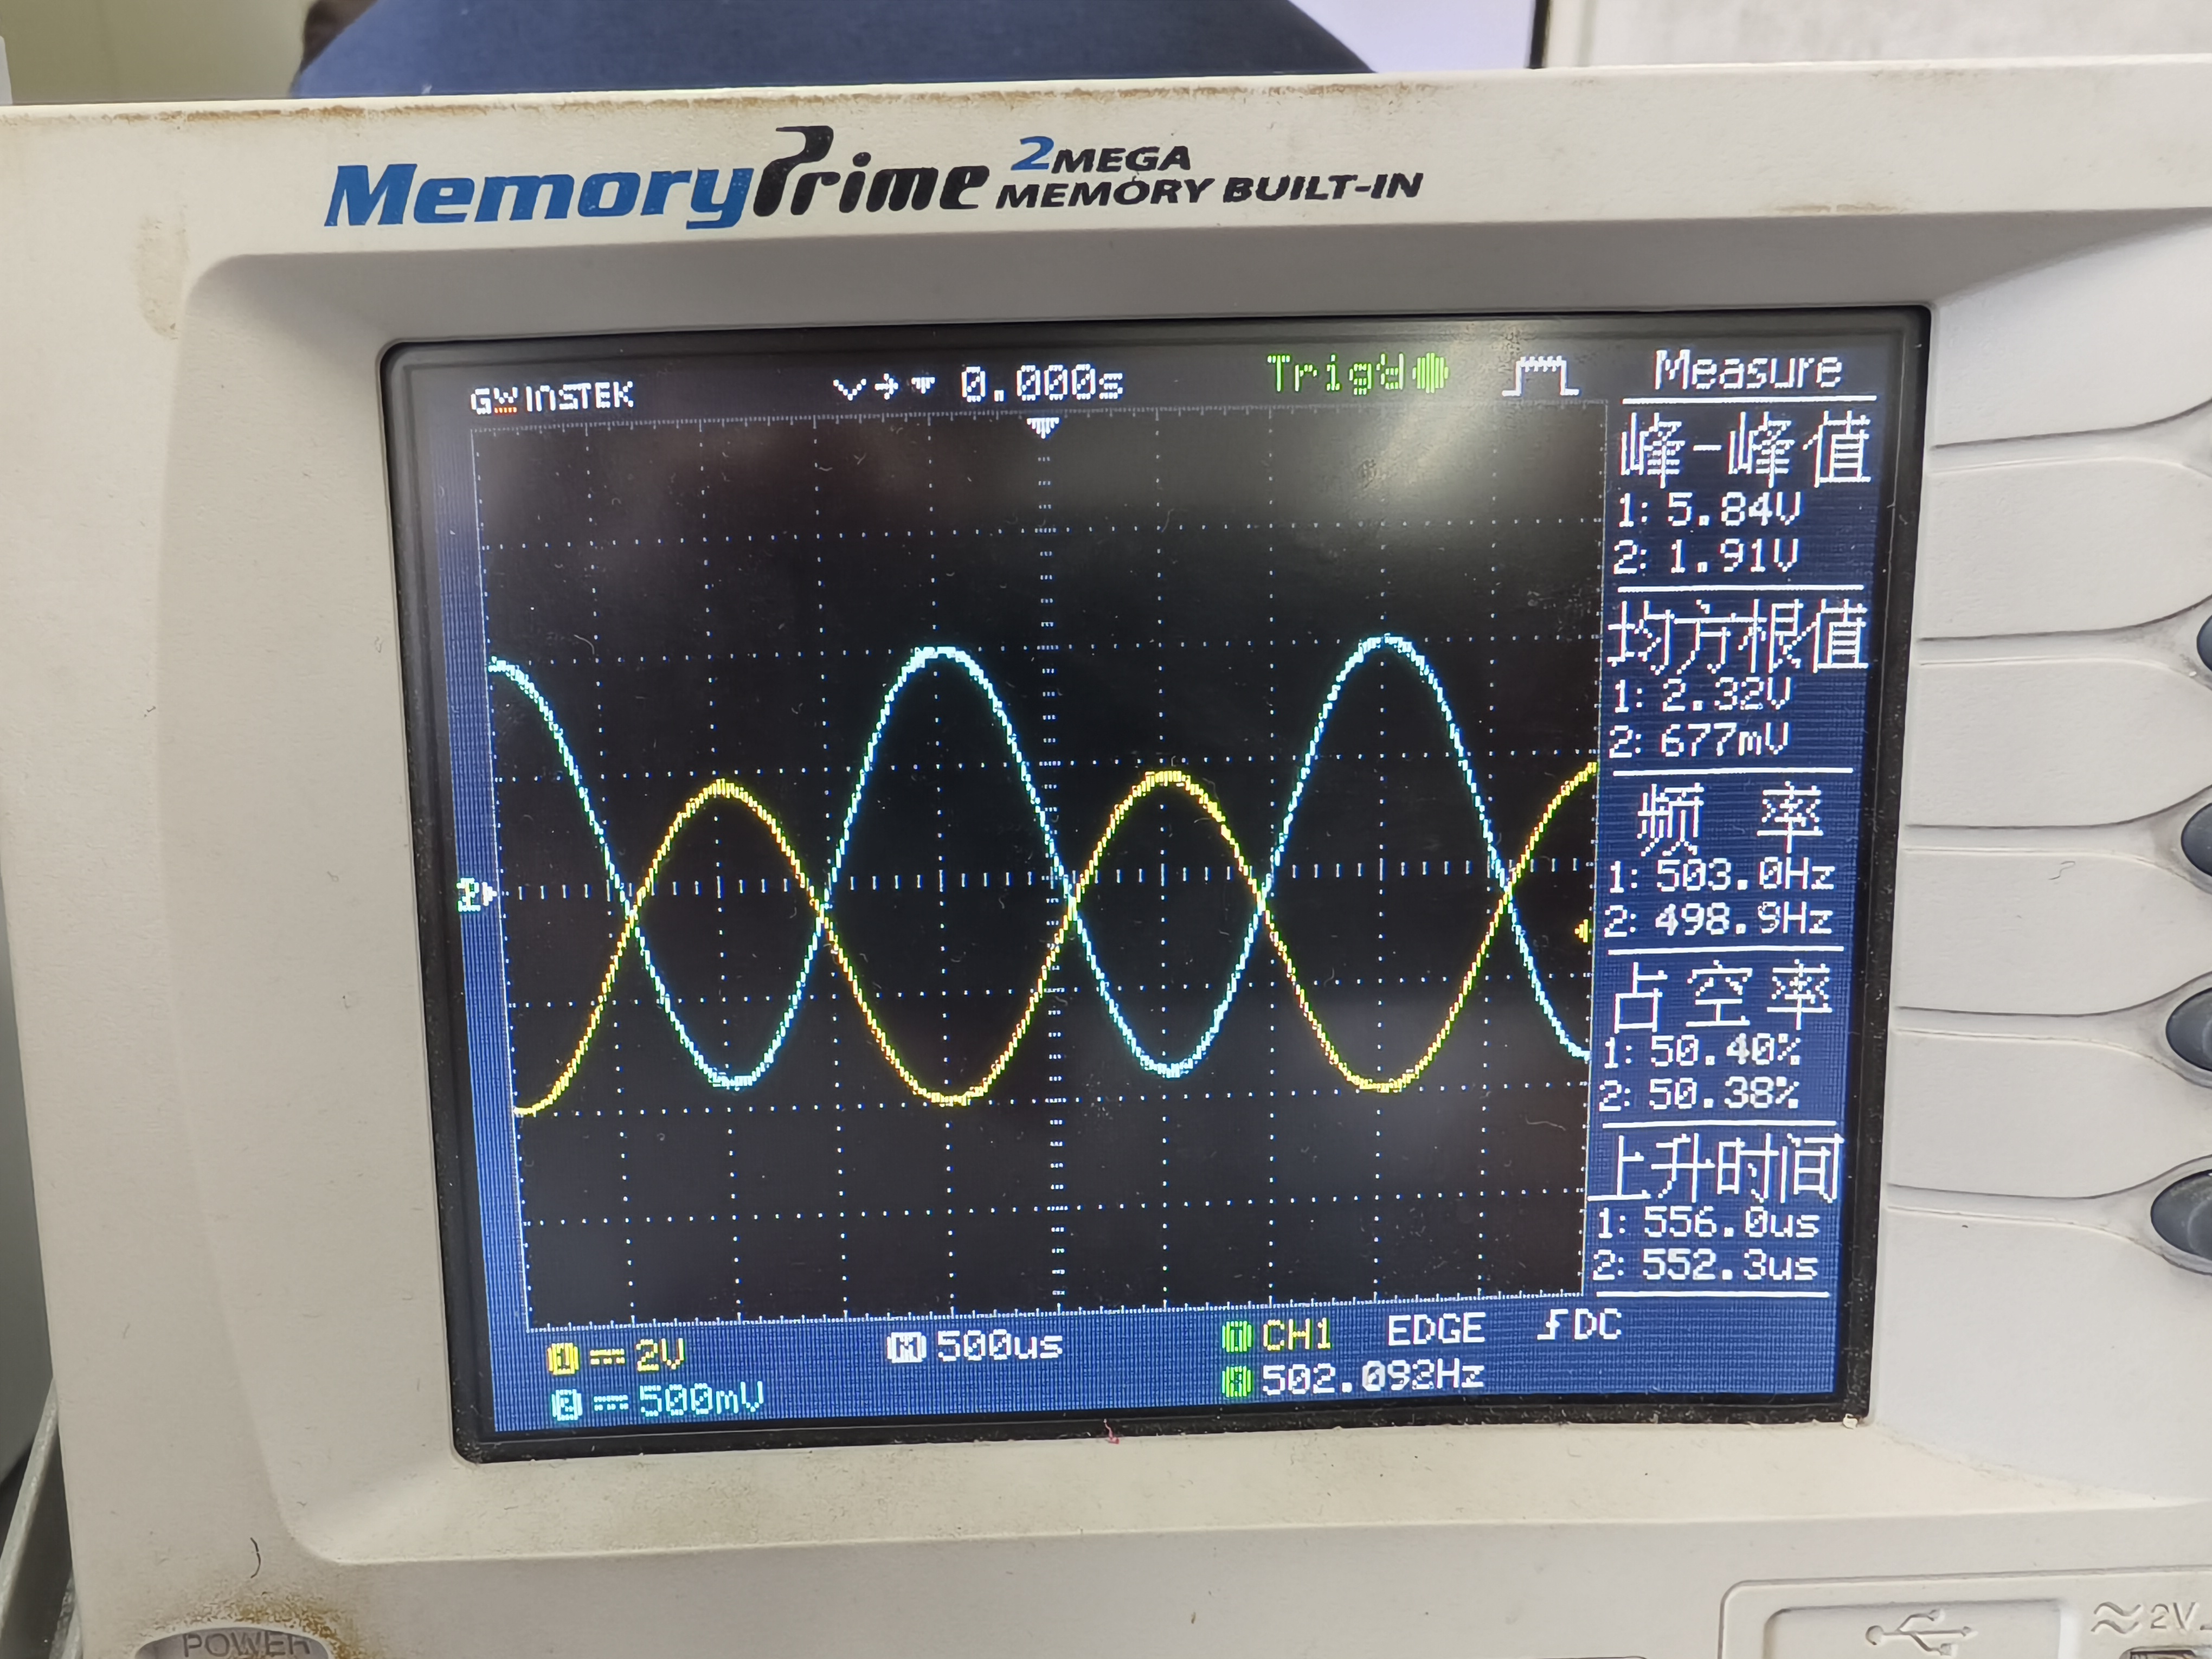
\includegraphics[width=1.0\textwidth]{image/3.jpg}
            \caption{反相加法器输出波形}
            \label{fig:反相加法器输出波形}
        \end{minipage}
        \hfill
        \begin{minipage}
    {0.45\textwidth}
            \centering
            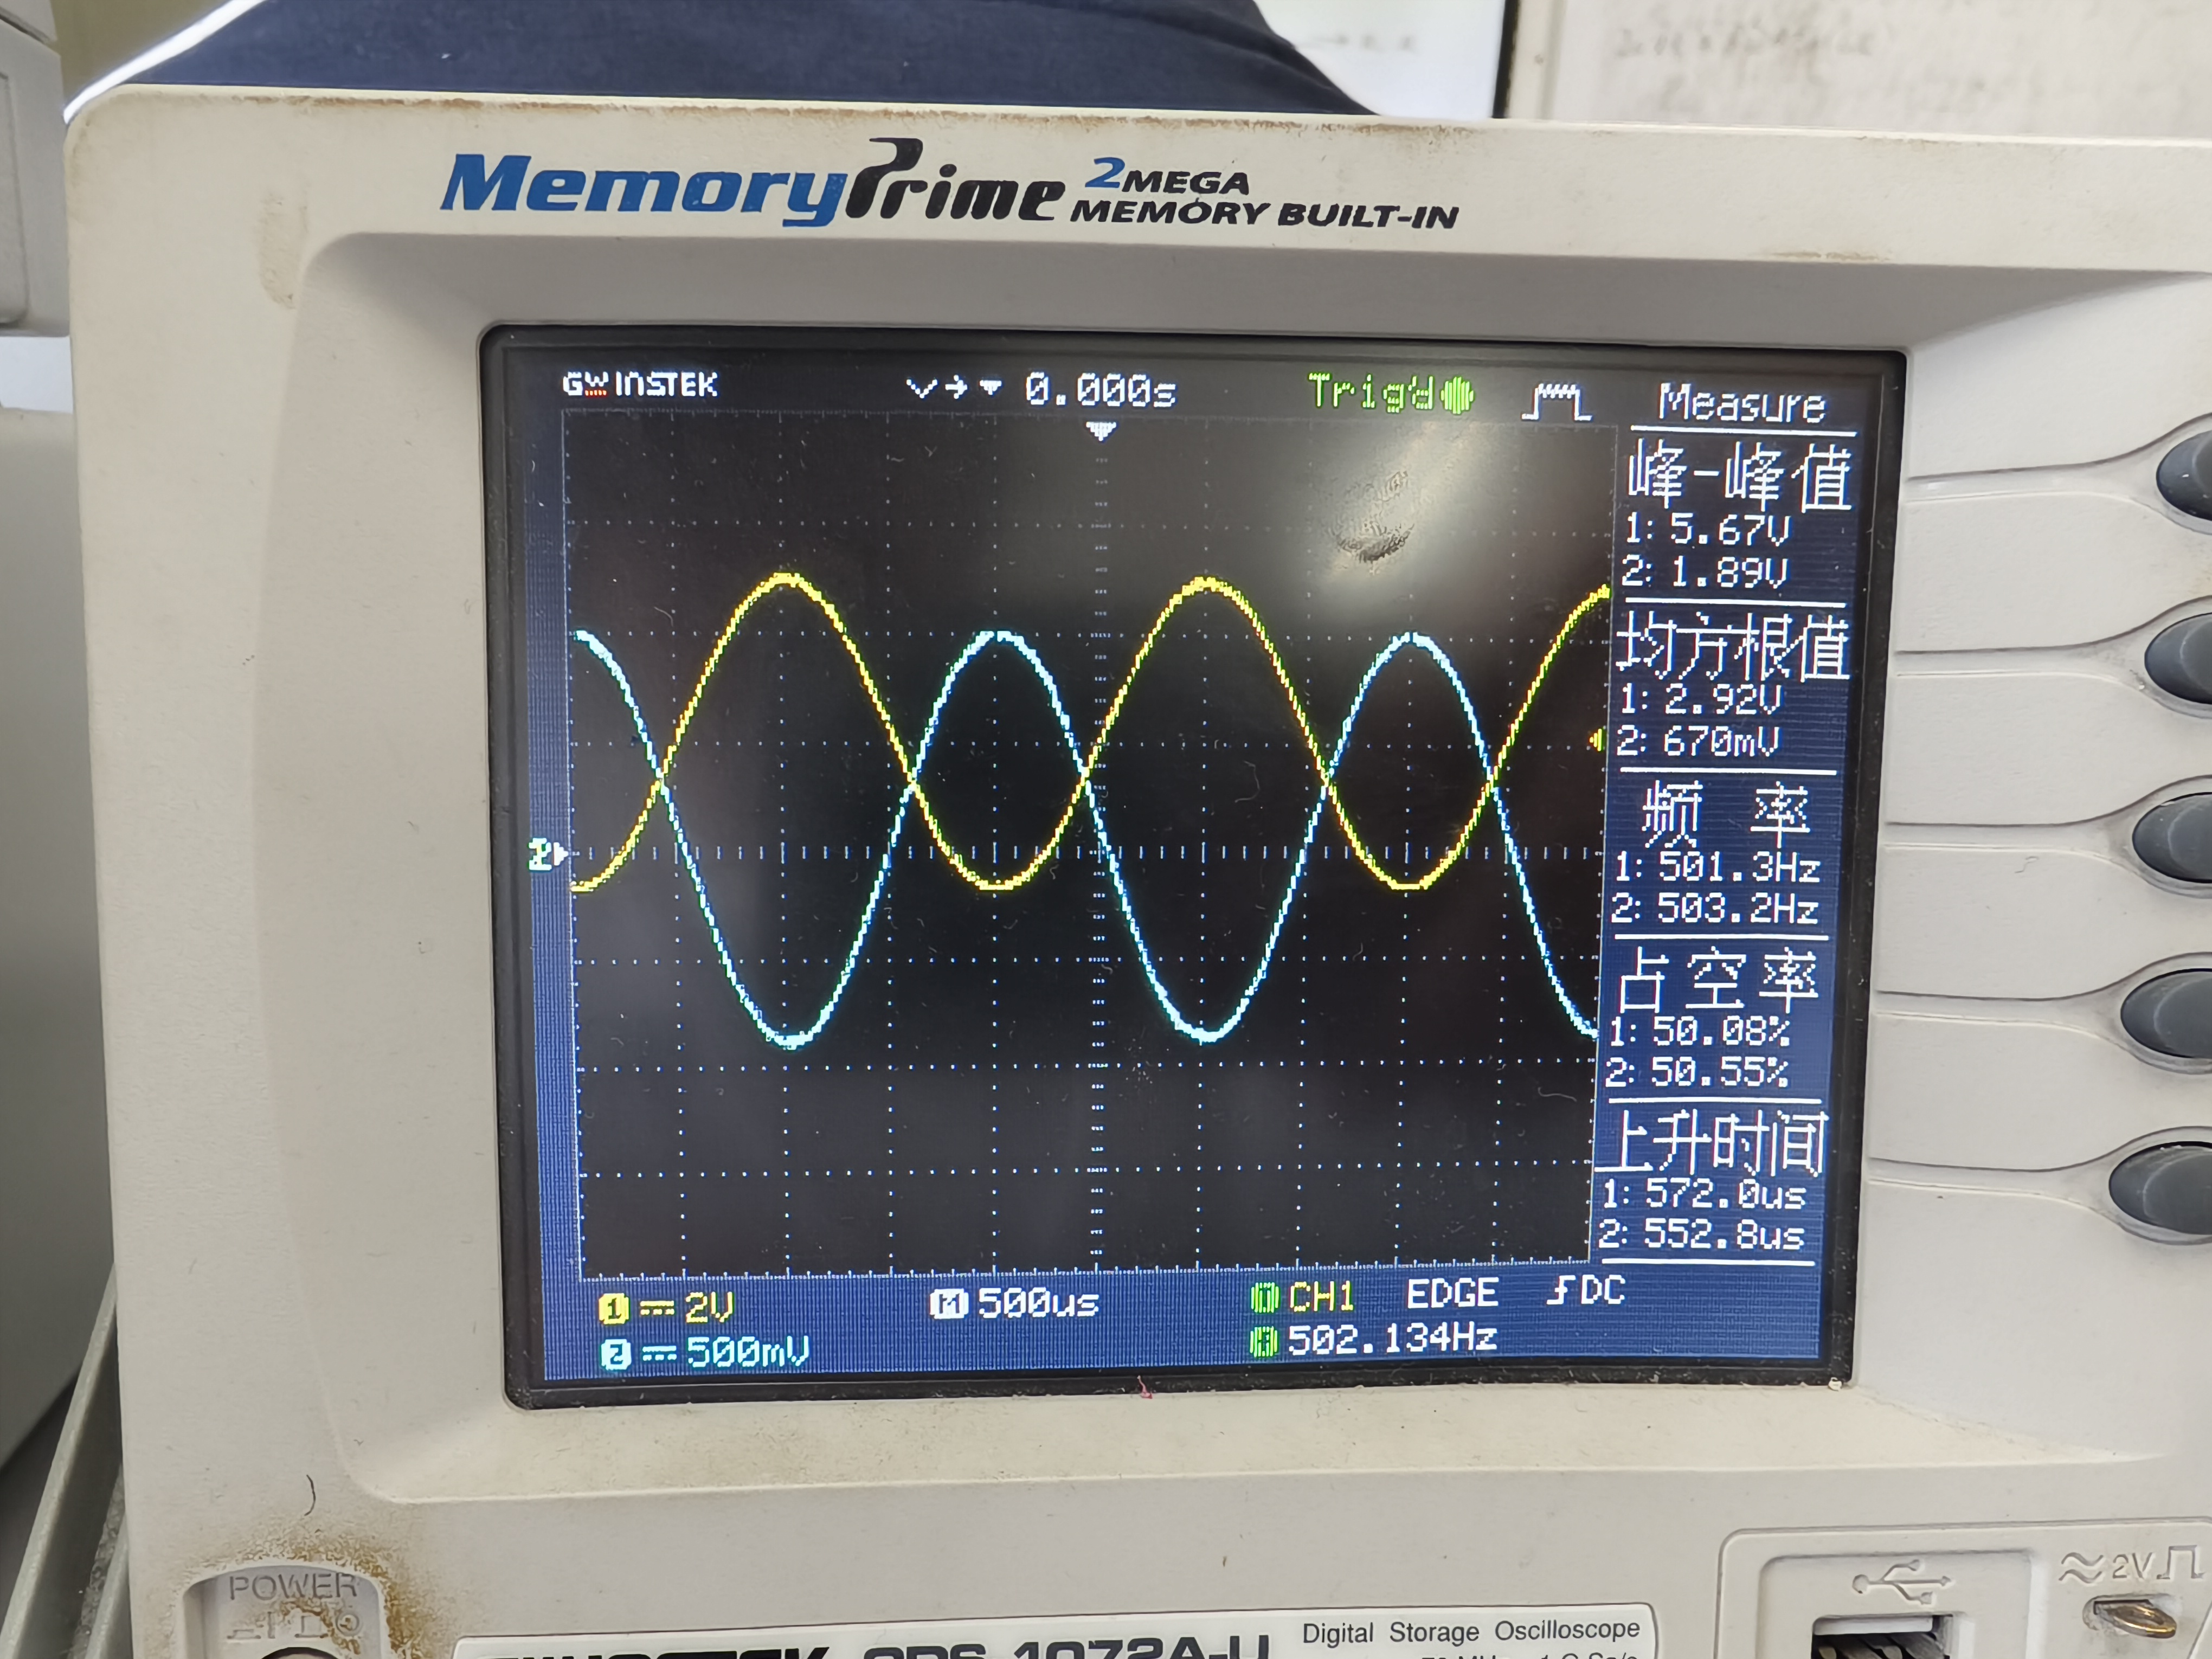
\includegraphics[width=1.0\textwidth]{image/4.jpg}
            \caption{同相加法器输出波形}
            \label{fig:同相加法器输出波形}
        \end{minipage}
\end{figure}

\subsection{实验结论}
……
\section{思考题}
\subsection{题面}
\begin{enumerate}[leftmargin=50pt,label=(\arabic*)] % 设置序号格式为(1)
    \item 减法运算电路中,若将输入信号$V_{12}$、$v_{11}$的输入端位置交换,输出将是什么样的?
    \item 若要将方波信号变成三角波信号,可选用哪一种运算电路?

\end{enumerate}
\subsection{回答}

\begin{enumerate}[leftmargin=50pt,label=(\arabic*)] % 设置序号格式为(1)
    \item 输出波形在电压轴上翻转
    \item 使用反相积分器
\end{enumerate}

\section{实验体会及建议}
\subsection{实验体会}
测量时应注意小心调试仪器, 尽量将读数稳定在误差允许范围内进行读数。
\subsection{建议}
注意电源正负极的接入, 防止反接造成仪器损坏, 注意正负电压的接入, 防止反接造成仪器损坏。

\end{document}
